\chapter{State of the Art} \label{chap:State of the Art}
Chapter Header

\section{Implementation of Reactive Systems}

\subsection{Observer Design Pattern}

\subsection{Reactive Programming}

\subsection{RxJs and BaconJs}

\begin{figure}[!h]
	\centering
	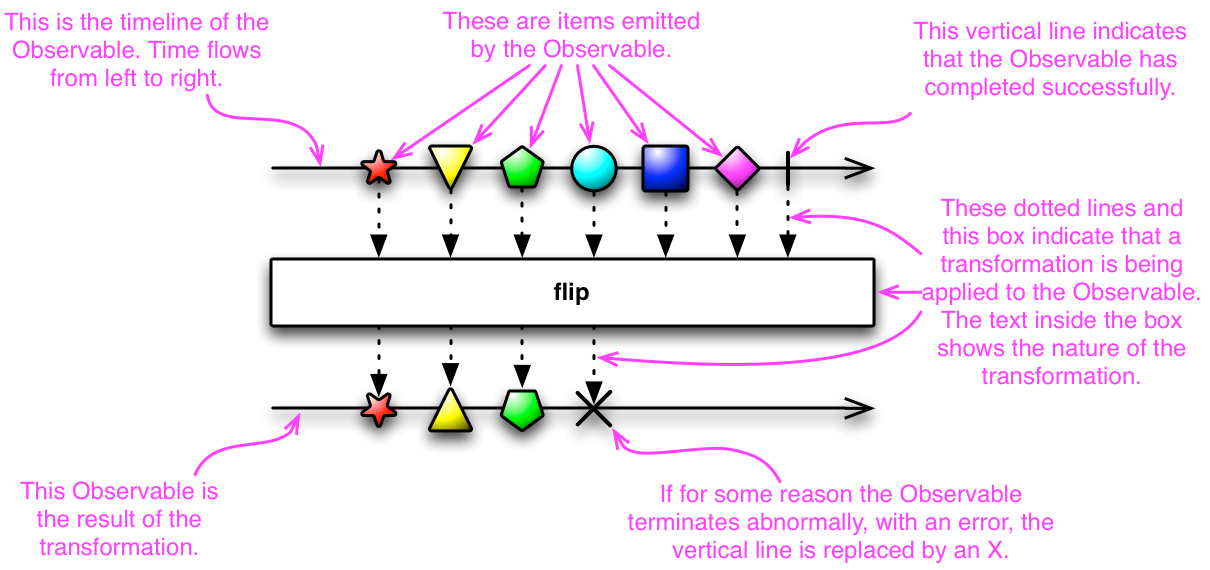
\includegraphics[scale=0.5,trim=0 0 0 0]{gfx/rxjs-reactive-pattern2.png}
	\caption{Reactive pattern \protect\cite{ReactiveXobservable}}
	\label{fig:rxjs-reactive-pattern}
\end{figure}

\textbf{Observable and Observer}\\
Placeholder

\textbf{Operators}
\label{subsec:Operators}\\

\textbf{RxJS Code Structure}\\
Placeholder
\begin{lstlisting}[language=JavaScript, caption=RxJS Simple Example, label={lst:RxJS_Simple_Example}]
// 1. Srouce Observable Creation
var sourceObservable = Rx.Observable.interval(1000);
// 2. Transformation by applying different operators
var transformedObservable = sourceObservable.map(function(x) {
		return x * 10;
	})
	.filter(function(x) {
		return x !== 20
	})
// OUTPUT
Next: 0
Next: 10
Next: 30
Next: 40
Next: 50
Completed
\end{lstlisting}

\subsection{Bacon.js}

\textbf{EventStream and Property}\\
Placeholder

\section{Debugging and Tools Support}

\subsection{Debugging JavaScript}

\subsection{Previous work on the Chrome Reactive Inspector}
	\subsubsection{Master Thesis by Waqas Abbas}
	\subsubsection{Master Thesis by Pradeep Baradur}
	\subsubsection{Merging efforts}
	% everything done by my predecessors in short, focus of both works and what differed

\section{Related Work}